% Author: Isaac H. Lopez Diaz
% Description: Presentation for current thesis project

\documentclass{beamer}

% Necessary imports
\usepackage{tikz}
\usetikzlibrary{shapes, automata, positioning, arrows, calc}
\usepackage{caption}
\usepackage{ulem}
\usepackage{verbatim}
\usepackage{graphicx}

% Document info
\title{Implementation of RAISE Specification Language (RSL)}
\author{Isaac H. Lopez Diaz\inst{1}}
\institute
{
\inst{1}
Department of Computer Science\\
University of Puerto Rico at Rio Piedras
}

%% DOC START %%
\begin{document}
\maketitle

% FRAME 1 %
\begin{frame}
\frametitle{What is RSL?}
\begin{itemize}
\item RAISE stands for ``Rigorous Approach to Industrial Software Engineering''.
\item It is a formal method specification language
\item If the specification is correct the code \sout{must be} is likely correct
\end{itemize}
\[ \text{check} : \text{Person} \times \text{Database} \rightarrow \text{Bool} \]
\[ \forall \text{p} : \text{Person}, \text{db} : \text{Database} \bullet \text{check(p, db)} \equiv \text{p} \in \text{db} \]
\end{frame}

% FRAME 2 %
\begin{frame}
  \frametitle{What is formal methods?}
  
\end{frame}

% FRAME 3 %
\begin{frame}
  \frametitle{What is model checking?}
\end{frame}


%% TIKZ func %% 
\tikzset{
	->,  % makes the edges directed
	>=stealth, % makes the arrow heads bold
	shorten >=2pt, shorten <=2pt, % shorten the arrow
	node distance=3cm, % specifies the minimum distance between two nodes. Change if n
	every state/.style={draw=blue!55,very thick,fill=blue!20}, % sets the properties for each ’state’ n
	initial text=$ $, % sets the text that appears on the start arrow
 }

% FRAME 4 %
\begin{frame}
\frametitle{Implementing a Interpreter \sout{Model Checker}}
\begin{figure}
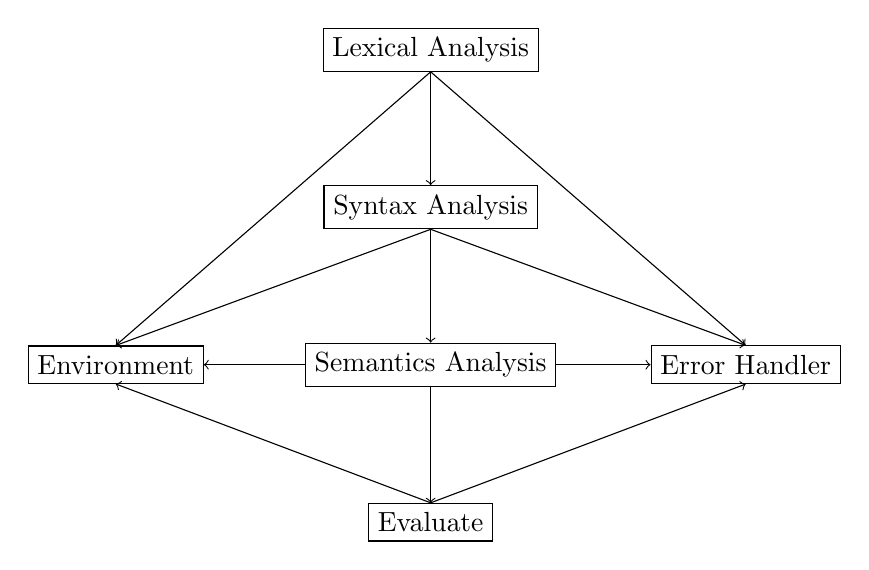
\begin{tikzpicture}
\node (la) at (4,0) [draw, rectangle] {Lexical Analysis};
\node (sa) at (4,-2) [draw, rectangle] {Syntax Analysis};
\node (err) at (8, -4) [draw, rectangle] {Error Handler};
\node (sm) at (4, -4) [draw, rectangle] {Semantics Analysis};
\node (env) at (0, -4) [draw, rectangle] {Environment};
\node (ev) at (4, -6) [draw, rectangle] {Evaluate};
\draw[->] (la.south) -- (sa.north);
\draw [->] (sa.south) -- (sm.north);
\draw [->] (sm.south) -- (ev.north);
\draw [->] (la.south) -- (env.north);
\draw [->] (la.south) -- (err.north);
\draw [->] (sa.south) -- (env.north);
\draw [->] (sa.south) -- (err.north);
\draw [->] (sm.west) -- (env.east);
\draw [->] (sm.east) -- (err.west);
\draw [->] (ev.north) -- (env.south);
\draw [->] (ev.north) -- (err.south);
\end{tikzpicture}
\caption{Interpreter phases}
\end{figure}
\end{frame}

% FRAME 5 %
\begin{frame}
  \frametitle{How to implement?}
  \begin{itemize}
  \item Using functional programming
  \item Standard lexing and parsing techniques
  \item Semantic analysis and type checker most difficult
  \item ... actually model checking
  \item Demo at end of presentation
  \end{itemize}
\end{frame}

% FRAME 6 %
\begin{frame}
  \frametitle{Why Lisp?}
  \begin{figure}
    \centering
    \includegraphics[scale=0.45]{lisp.png}
    \caption{Lisp mascot}
    \label{fig:enter-label}
  \end{figure}
  
  \begin{itemize}
  \item (Easy to represent expressions)
  \item (Easy to alter state '(unlike Haskell))
  \item (Easy to do symbolic computation)
  \item (Programming in Lisp is fun!)
  \end{itemize}
\end{frame}

% FRAME 7 %
\begin{frame}
  \frametitle{Example: Weakest Precondition (or Predicate Calculus)}
  Given some statement \textit{S} and a \textbf{postcondition} \textit{R},
  the \textbf{weakest precondition} is a predicate \textit{Q} such that for
  any \textbf{precondition} \textit{P} \( \{P\} S \{R\} \Longleftrightarrow P \Rightarrow Q \)
  \begin{itemize}
  \item \(wp(\textbf{skip}, R) = R\)
  \item \(wp(\textbf{abort}, R) = False\)
  \item \(wp(\textbf{x := E}, R) = R[x \leftarrow E] \)    
  \end{itemize}
\end{frame}

% REFERENCES
\begin{frame}[allowframebreaks]
  \frametitle{References}
\nocite*
\bibliographystyle{acm}
\bibliography{refs}
\end{frame}
\end{document}
%% DOC END %%
